\section{Технические характеристики линий передаич данных} %9

\subsection{Описание адаптированного IPv6 уровня} %9.4
 
\subsubsection{Ввод в эксплуатацию новых устройств} %9.4.4

Расширение к приложению Е % 9.4.4.2

Формат сообщений протокола начальной загрузки LoWPAN (LBP) % 9.4.4.2.1

Встроенные сообщения EAP % 9.4.4.2.1.2

LBM сообщения вкладывают особые аутентификационные сообщения (EAP) описанные в IETF RFC 3748. На рисунке \ref{img:9-23} представлены изменения, необходимые для соответствия информационным LBP элементам. В таблице 1 описаны поля сообщения.  %\ref{tab:9-48}

\begin{figure}[h]
 \label{img:9-23}
 \center{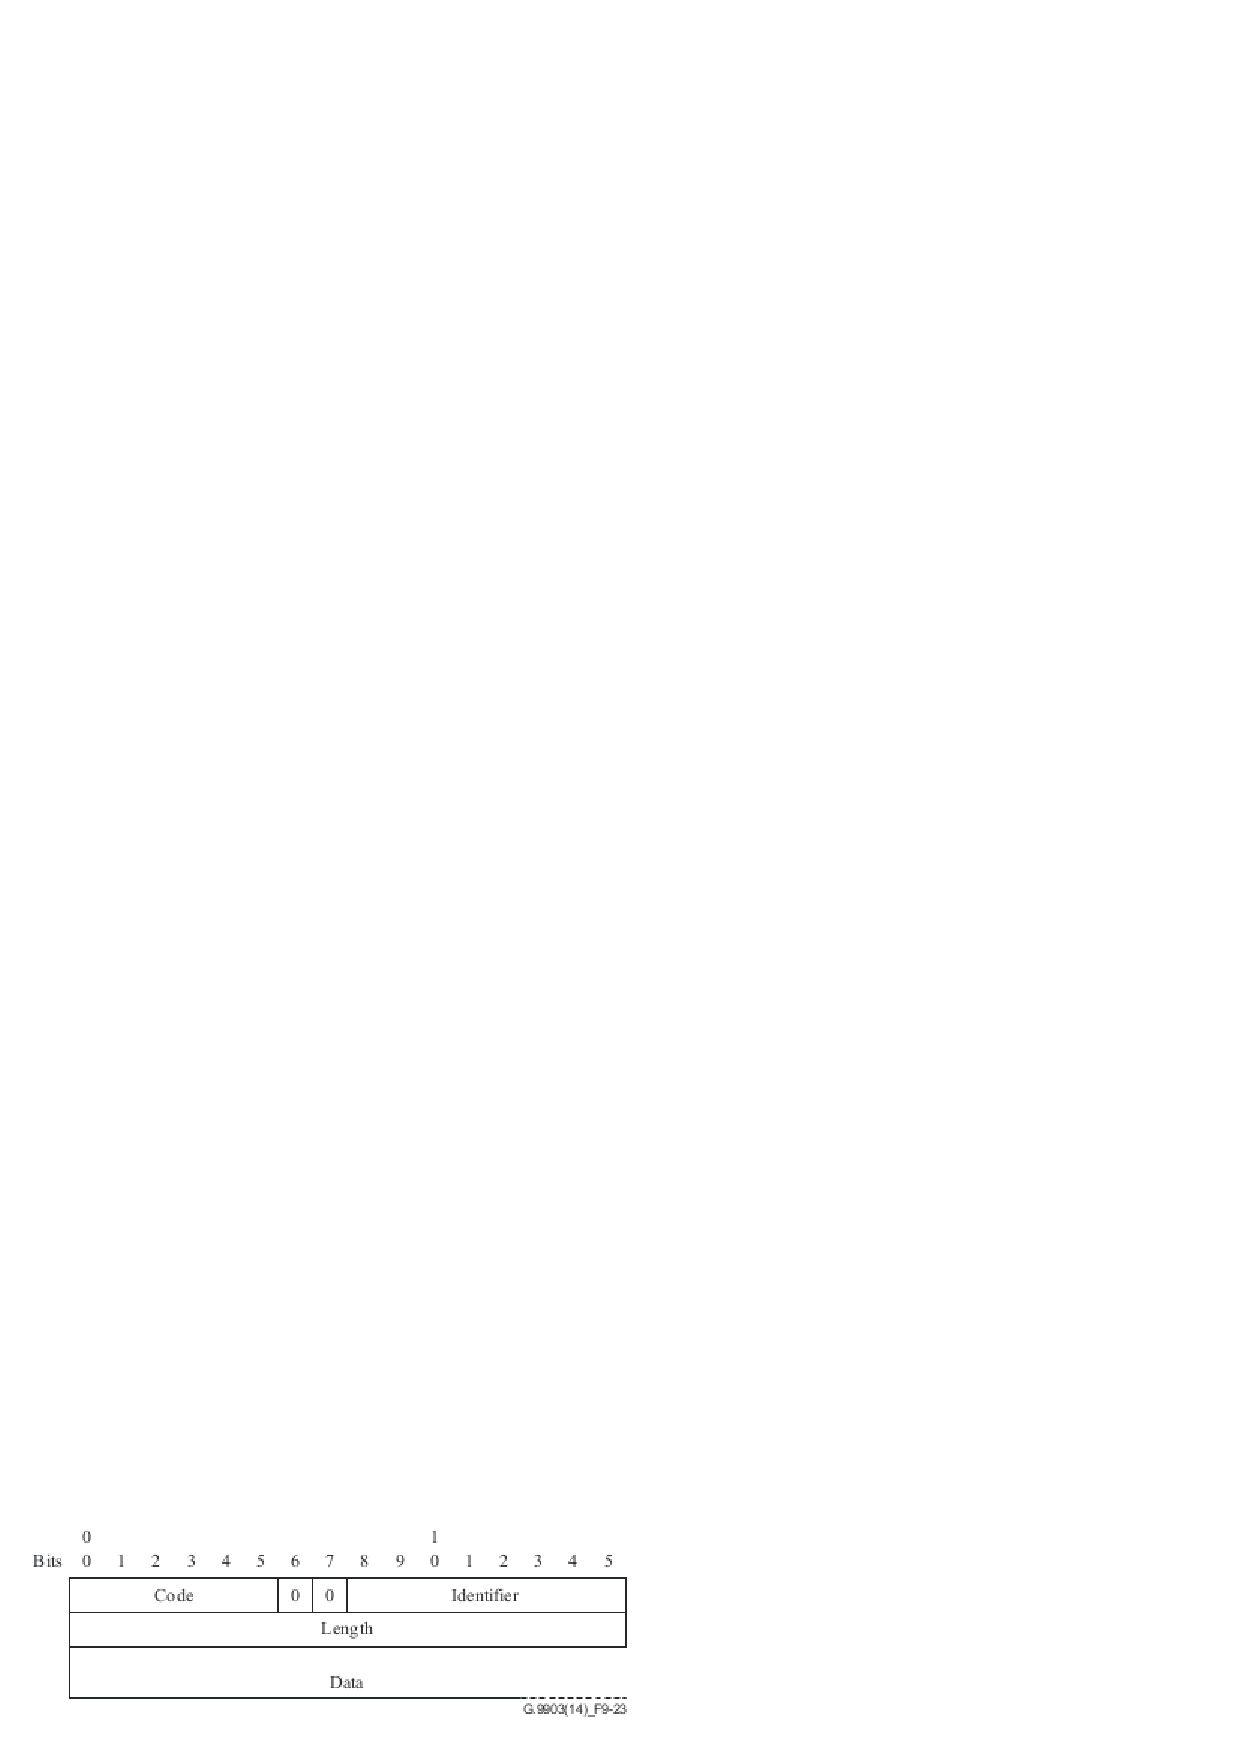
\includegraphics{pictures/9-23}}
 \caption{Общий формат EAP сообшения}
\end{figure}

\begin{longtable}[\textwidth]{|p{0.21\linewidth}|p{0.15\linewidth}|p{0.64\linewidth}|}
\caption{Поля, встроенные в EAP сообшение} \\ % \ref{tab:9-48}
\hline
Поле & Размер & Описание \\ \hline
Код & 6 бит & Определяет тип EAP покета. Каждый код соответствует: \\
& & 0b000001: Запрос (клиентк отправлен LBP) \\
& & 0b000010: Ответ (получен от клиента) \\
& & 0b000011: Успех (отправления клиенту) \\
& & 0b000100: Неудача (отправления клиенту) \\
& & Поле кода отличается от стандартного поля кода EAP. Существует простое двустороннее преобразование описанное в IETF RFC 3748. Преобразование провизводится если происходит передача покета по другому протоколу (например RADIUS) и в случае контроля целостности EAP заголовка. \\ \hline
Идентификатор &  8 бит & Помогает при согласовании ответа с запросом. \\ \hline
Длина & 16 бит & Указывает размер пакета в байтах. Включает в себя поле кода, идентификатора, длины и поля данных. Сообщения, с длиной, меньше указанной в поле, должны игнорироваться. \\ \hline
Данные & переменная длина & Формат поля данных опрелеляется полем кода. Больше информации в IETF RFC 3748 \\ \hline
\end{longtable}
